\documentclass[12pt, openany]{book}

% ──────────────────────────────────────────────
% Packages
% ──────────────────────────────────────────────
\usepackage[margin=1in]{geometry}
\usepackage{amsmath, amssymb, amsthm}
\usepackage{mathtools}
\usepackage{bm}
\usepackage{graphicx}
\usepackage{tikz}
\usepackage{pgfplots}
\pgfplotsset{compat=1.18}
\usetikzlibrary{arrows.meta, decorations.markings, calc, patterns, positioning}
\usepackage{tcolorbox}
\tcbuselibrary{theorems, breakable, skins}
\usepackage{hyperref}
\usepackage{enumitem}
\usepackage{fancyhdr}
\usepackage{titlesec}
\usepackage{epigraph}
\usepackage{xcolor}
\usepackage{booktabs}

% ──────────────────────────────────────────────
% Colors
% ──────────────────────────────────────────────
\definecolor{chapblue}{RGB}{0, 70, 130}
\definecolor{accentred}{RGB}{180, 40, 40}
\definecolor{softgray}{RGB}{245, 245, 245}
\definecolor{trajgreen}{RGB}{30, 130, 60}
\definecolor{darkgold}{RGB}{160, 120, 20}
\definecolor{purplehaze}{RGB}{100, 40, 140}

% ──────────────────────────────────────────────
% Theorem environments
% ──────────────────────────────────────────────
\newtcbtheorem[number within=chapter]{principle}{Principle}{
  colback=chapblue!5, colframe=chapblue!80,
  fonttitle=\bfseries, separator sign={.~},
  breakable
}{princ}

\newtcbtheorem[number within=chapter]{keyidea}{Key Idea}{
  colback=accentred!5, colframe=accentred!70,
  fonttitle=\bfseries, separator sign={.~},
  breakable
}{idea}

\newtcbtheorem[number within=chapter]{example}{Example}{
  colback=softgray, colframe=black!40,
  fonttitle=\bfseries, separator sign={.~},
  breakable
}{ex}

\newtcbtheorem[number within=chapter]{definition}{Definition}{
  colback=darkgold!5, colframe=darkgold!80,
  fonttitle=\bfseries, separator sign={.~},
  breakable
}{def}

\newtcbtheorem[number within=chapter]{remark}{Remark}{
  colback=purplehaze!5, colframe=purplehaze!60,
  fonttitle=\bfseries, separator sign={.~},
  breakable
}{rem}

\newtcbtheorem[number within=chapter]{warning}{Warning}{
  colback=accentred!5, colframe=accentred!80,
  fonttitle=\bfseries, separator sign={.~},
  breakable
}{warn}

\theoremstyle{plain}
\newtheorem{proposition}{Proposition}[chapter]
\newtheorem{theorem}{Theorem}[chapter]
\newtheorem{lemma}[theorem]{Lemma}
\newtheorem{corollary}[theorem]{Corollary}

% ──────────────────────────────────────────────
% Chapter formatting
% ──────────────────────────────────────────────
\titleformat{\chapter}[display]
  {\normalfont\huge\bfseries\color{chapblue}}
  {\chaptertitlename\ \thechapter}{20pt}{\Huge}
\titlespacing*{\chapter}{0pt}{-20pt}{30pt}

% ──────────────────────────────────────────────
% Header/Footer
% ──────────────────────────────────────────────
\pagestyle{fancy}
\fancyhf{}
\fancyhead[LE,RO]{\thepage}
\fancyhead[RE]{\textit{Control Is Motion}}
\fancyhead[LO]{\textit{\nouppercase{\leftmark}}}
\renewcommand{\headrulewidth}{0.4pt}
\setlength{\headheight}{14.5pt}

% ──────────────────────────────────────────────
% Custom commands
% ──────────────────────────────────────────────
\newcommand{\state}{\bm{x}}
\newcommand{\control}{\bm{u}}
\newcommand{\traj}{\bm{\gamma}}
\newcommand{\manifold}{\mathcal{M}}
\newcommand{\configspace}{\mathcal{Q}}
\newcommand{\statespace}{\mathcal{X}}
\newcommand{\controlspace}{\mathcal{U}}
\newcommand{\Reals}{\mathbb{R}}
\newcommand{\dd}{\mathrm{d}}
\newcommand{\dt}{\,\dd t}
\newcommand{\norm}[1]{\left\lVert #1 \right\rVert}
\newcommand{\inner}[2]{\left\langle #1,\, #2 \right\rangle}

% ──────────────────────────────────────────────
\begin{document}

\setcounter{chapter}{6}

\chapter{Funnel Synthesis}
\label{ch:funnel_synthesis}

\section{What Must Survive a Perturbation?}

A nominal swing answers one question: can this model, with these inputs, produce this motion and impact? A feedback calculation asks how nearby deviations evolve. A funnel asks a stronger, explicitly bounded question: which sets of initial states and disturbances can this particular controller accommodate while respecting the declared task? These are successive investigations, not interchangeable descriptions of athletic skill. A beautifully shaped tube is useful only when its boundary follows from the equations, its inputs are realizable, and its terminal states meet the actual impact requirements.

The distinction matters for golf. Clubhead speed, face orientation, strike location, and arrival time are coupled outputs of a constrained mechanical system. The same change in wrist motion can alter several of them, while a deviation that looks large in one joint coordinate may scarcely change the selected impact output. Conversely, a small deviation in a sensitive direction can matter greatly. A funnel can organize those dependencies for a specified model. Its shape alone does not establish a golfer's nervous-system strategy, a universal release pattern, or a measured tolerance for error.

The preceding chapters supplied feasible trajectories, local transverse dynamics, finite-horizon feedback, and candidate uncertainty models. None automatically supplies a nonlinear invariance certificate. In particular, a positive Riccati solution can define level sets that expand in physical coordinates. Expansion is compatible with containment when the actual motion expands more slowly. Contraction, set containment, bounded input, and terminal accuracy must each be checked rather than inferred from the word ``funnel.''

\section{A Moving Set and Its Boundary Condition}

Consider a closed-loop model $\dot x=f(x,k(x,t),t,w)$ on a declared state domain, with admissible disturbance $w\in\mathcal W$. Let $x_d(t)$ be a differentiable reference, and put $e=x-x_d(t)$. Its exact error dynamics are
\begin{equation}
 F(e,t,w)=f(x_d(t)+e,k(x_d(t)+e,t),t,w)-\dot x_d(t).
 \label{eq:funnel_exact_error}
\end{equation}
If the nominal reference is infeasible, the residual $F(0,t,0)$ does not vanish. Dropping that residual creates a certificate for a different model. Actuator states, state-estimation errors, or delay approximations belong in $x$ when they influence the realized feedback; a controller that sees the true state instantly cannot certify an implementation that does not.

Choose a differentiable scalar $V(e,t)$ and a positive level $\rho(t)$ on a finite interval $[0,T]$. Define
\begin{equation}
 \mathcal F(t)=\{e:g(e,t)=V(e,t)-\rho(t)\leq0\},\qquad
 q(e,t,w)=V_t+\nabla_e V^\top F-\dot\rho.
 \label{eq:funnel_boundary_derivative}
\end{equation}
A sufficient invariance condition is $q\leq0$ on $g=0$, for every allowed disturbance and every time in the interval, under the regularity assumptions below. The subtraction of $\dot\rho$ is essential: the boundary moves too. A strict margin $q\leq-\varepsilon$, with $\varepsilon>0$, gives an inward-pointing certificate where it is feasible. Strictness is stronger than invariance and should not be claimed from mere nonnegativity of an optimization expression.

For the usual boundary argument, take $V,\rho$ continuously differentiable, a regular boundary $\nabla_e g\neq0$, and error dynamics continuous in their arguments and locally Lipschitz in $e$, uniformly over the allowed disturbance set. Assume measurable disturbances, well-defined solutions, and compact tubes contained in a model domain on which the required existence and uniqueness conditions hold through $T$. For a continuous differential inclusion obtained by allowing all $w\in\mathcal W$, the corresponding tangent condition must hold for every allowed velocity. These hypotheses rule out escape caused by a missing solution, a singular coordinate chart, or a nonunique evolution. Piecewise smooth dynamics and resets need their own interval and jump conditions.

To understand the proof, view $(e,t)$ as an extended state with $\dot t=1$. At a regular side boundary, $q$ is the derivative of its defining function along every allowed velocity. The inequality says that these velocities belong to the tangent half-space of the closed moving set. The standard invariance theorem then prevents outward crossing before the end of the interval. With a strict inward margin, a first-exit contradiction gives the familiar intuitive argument. The terminal slice $t=T$ ends the claim; this finite certificate is not an assertion about all future time.

Positive-definite $V$ is convenient for a tube centered on a reference, but the boundary condition itself is a containment argument. It does not require every interior value of $V$ to decrease, nor does it prove convergence to $e=0$. Conversely, checking $\dot V<0$ at a handful of interior states does not check the moving boundary. Safety and input conditions must hold throughout the tube, not just on its boundary.

\subsection{An Exact Robust Tube That Can Widen}

For the scalar model $\dot e=-ke+d$, with $k>0$ and $|d(t)|\leq\bar d$, choose $\mathcal F(t)=[-r(t),r(t)]$, where $r_0>0$. At $e=r$, the largest outward velocity is $-kr+\bar d$; the lower boundary gives the same condition. The choice
\begin{equation}
 \dot r=-kr+\bar d,\qquad
 r(t)=r_0e^{-kt}+\frac{\bar d}{k}(1-e^{-kt})
 \label{eq:funnel_scalar_radius}
\end{equation}
therefore contains every solution starting in the initial interval. Equivalently, $V=e^2$, $\rho=r^2$, and the worst boundary derivative $q$ is zero. Constant extreme disturbances attain the appropriate boundary solution, so this is an exact scalar bound, not just a Monte Carlo envelope.

When $r_0>\bar d/k$, the interval narrows. When $r_0<\bar d/k$, it widens. Both are valid. Persistent bounded disturbance prevents a guarantee of arbitrarily small asymptotic error for this controller. Even without disturbance, $e(t)=e_0e^{-kt}$ does not reach zero at a finite time from a nonzero initial error. Exponential attraction cannot be silently upgraded to an exact finite-time impact constraint.

Input limits further change the conclusion. If the same plant is an integrator with $u=-\operatorname{sat}(ke)$ and $|u|\leq\bar u$, its robust symmetric radius must satisfy $\dot r\geq-\min(kr,\bar u)+\bar d$. When $\bar d>\bar u$, no fixed finite interval is robustly invariant for this plant: an allowed constant disturbance can exceed the available opposing control. Increasing the requested feedback gain does not remove saturation. A widening finite-horizon bound can still be useful, provided it remains within the terminal and safety requirements.

\begin{figure}[htbp]
 \centering
 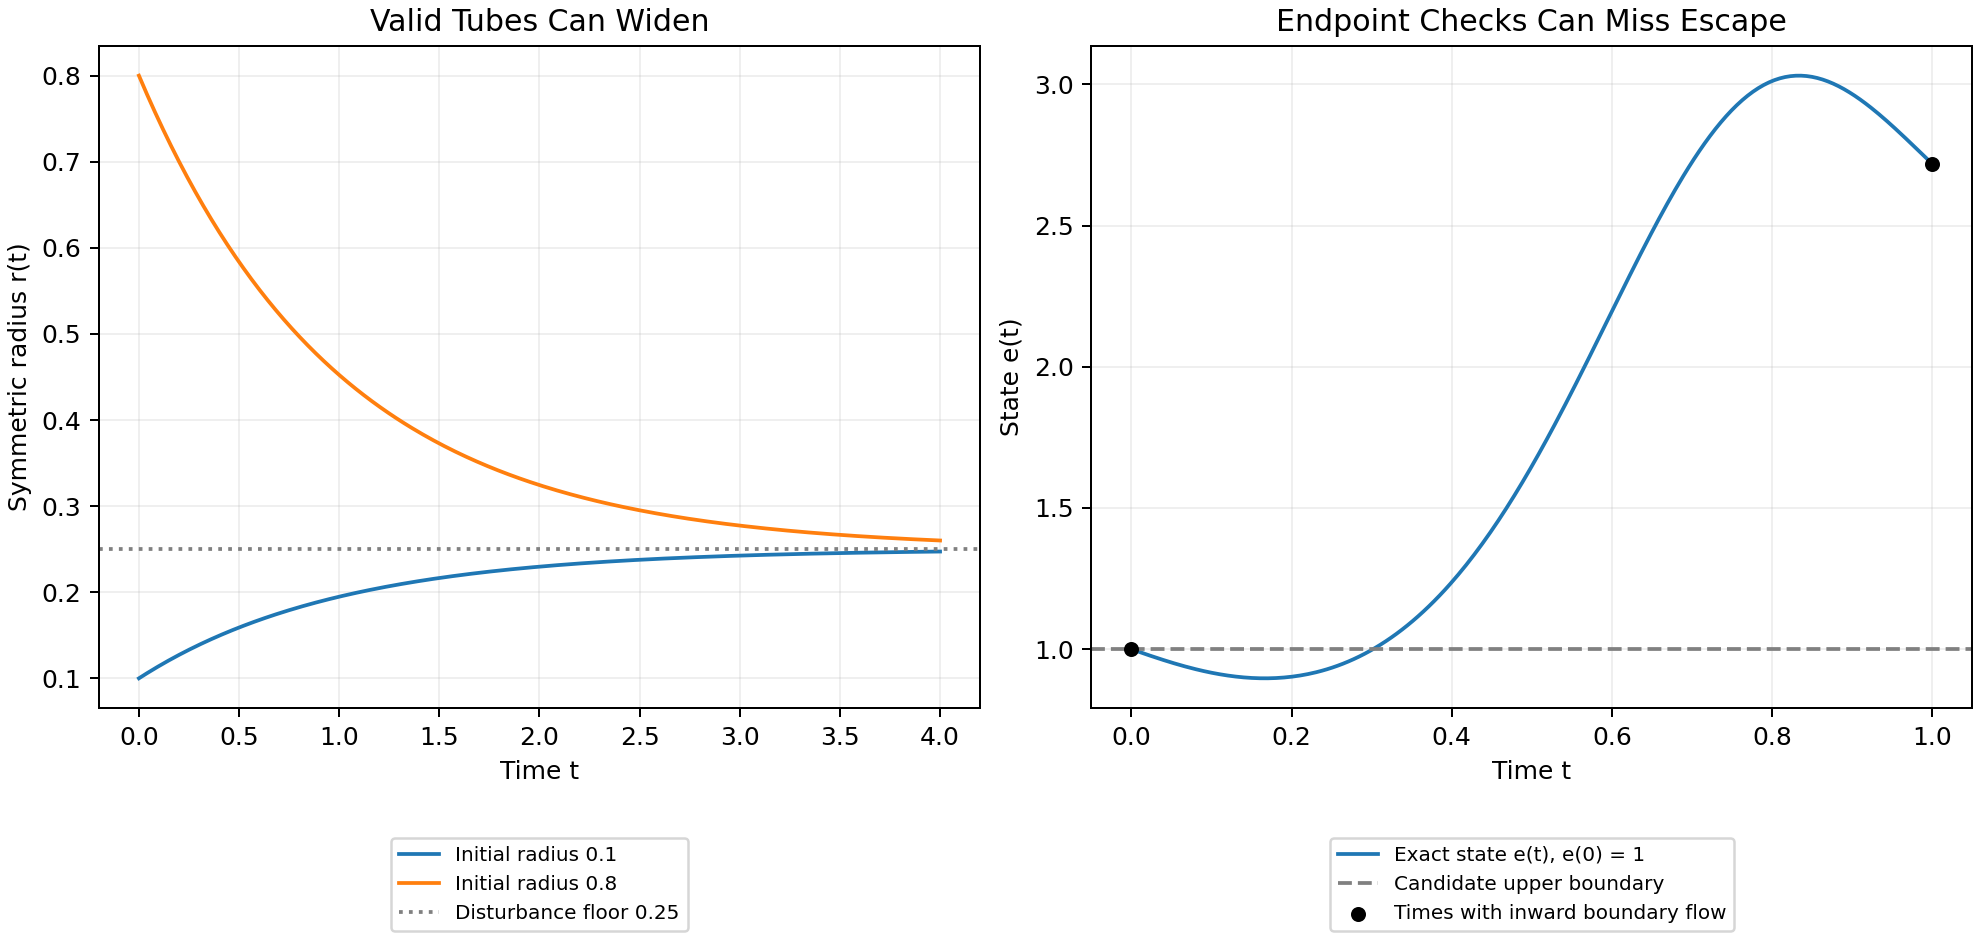
\includegraphics[width=\linewidth]{../The_Geometry_of_Motion/figures/funnel_invariance_examples.png}
 \caption{Containment Does Not Require Narrowing}
 \label{fig:funnel_invariance_examples}
\end{figure}

The left panel shows the exact scalar radius for $k=1$, $\bar d=0.25$, and two initial radii. The right panel shows a different system whose boundary appears inward-pointing at both sampled endpoints but escapes between them. Both panels are calculated model examples; neither is a fitted golf-swing funnel.

\section{Containment, Arrival, and Successful Impact}

Suppose the safe state set is $\mathcal S(t)$, the admissible input set is $\mathcal U$, and the terminal goal is $\mathcal G$. A timed reach-and-stay-inside claim requires $x_d(t)+\mathcal F(t)\subseteq\mathcal S(t)$ and $k(x_d(t)+e,t)\in\mathcal U$ for all $e\in\mathcal F(t)$, plus the terminal inclusion $x_d(T)+\mathcal F(T)\subseteq\mathcal G$. Together with invariance and existence, these conditions imply arrival in $\mathcal G$ at $T$ for the admitted initial states and disturbances. Invariance alone supplies none of the other inclusions.

A smooth finite-time flow with unique forward and backward local solutions maps open sets to open sets. It cannot map a full-dimensional open set of initial states exactly onto a lower-dimensional equality target at one prescribed finite time. This explains why a nondegenerate smooth timed tube generally terminates in a tolerance region rather than an exact state equality. Hybrid resets, nonsmooth finite-time controllers, and stopping at a state-dependent event change the assumptions and require separate analysis. A candidate $\rho(T)=0$ also destroys the regular nondegenerate boundary assumed above; it cannot be justified by simply substituting zero into the same theorem.

Golf impact is usually an event. A guard $h(x,t)=0$ describes contact, while a separate output $H(x,t)$ describes face orientation, impact location, relative velocity, or another performance variable. The equation $h=0$ does not guarantee desirable values of $H$. An event-based certificate needs no premature invalid contact, finite arrival at the intended guard, an appropriate crossing direction, and containment of $H$ in the allowed impact-output set at every admissible crossing. A guard can be reached accurately in its normal direction while the ball is struck with an unacceptable face angle or tangential offset.

One way to prove progress uses a valid phase coordinate $\tau$ with $\dot\tau=\nu\geq\nu_{\min}>0$ until the desired terminal phase. Then an initial phase gap $\Delta\tau$ is traversed within $\Delta\tau/\nu_{\min}$, provided the phase domain remains valid and the target phase actually represents the intended event. A phase tube $V(\xi,\tau)\leq\rho(\tau)$ must satisfy
\begin{equation}
 \nabla_\xi V^\top F_\xi+(V_\tau-\rho'(\tau))\nu\leq0
 \quad\hbox{on }V=\rho.
 \label{eq:funnel_phase_condition}
\end{equation}
Changing the coordinate to phase does not remove time from the physics. The phase speed, actuator bandwidth, disturbance specification, and event/reset conditions remain relevant. If $\nu$ can vanish or change sign, the progress bound fails, and division by $\nu$ is not legitimate throughout the tube.

\subsection{Which Set Is Being Approximated?}

For a fixed controller and initial uncertainty set, the forward reachable set contains all states generated by the allowed initial conditions and disturbances. An invariant funnel containing that initial set is an outer bound on this forward reachable set at each time. A smaller outer tube can make obstacle or safety checks less conservative.

For a fixed terminal goal, a different question asks which initial states can be brought to the goal while remaining admissible. A verified funnel with terminal inclusion gives an inner subset of this backward feasible set for the chosen policy. Relative to a problem allowing other admissible policies, it is still a sufficient subset, provided the controller has the same information and disturbance rules as that problem. Expanding its initial slice may increase the set of initial conditions certified as recoverable. Minimizing a forward uncertainty envelope and maximizing an initial capture set are different optimization objectives, not conflicting descriptions of one volume calculation.

An optimal value function is another object. It depends on a specified cost, terminal condition, control class, and treatment of uncertainty. For a deterministic cost-minimization problem, the Hamilton--Jacobi--Bellman equation, interpreted appropriately when the solution is nonsmooth, relates that value to the optimal policy. Its finite sublevel sets can describe cost-bounded feasible states when the boundary data encode the goal. An arbitrary Lyapunov polynomial is not automatically a value-function approximation or a cost bound. Invariance is a feasibility statement only after the other task conditions are supplied.

For a concrete cost comparison, let the realized policy have running cost $L(x,k,t)$ and terminal cost $\phi(x(T))$. If a differentiable function $W$ satisfies $W_t+\nabla W^\top f+L\leq0$ along all admitted trajectories and $W(x,T)\geq\phi(x)$ on their terminal set, integration gives
\begin{equation}
 \int_t^T L(x(s),k(x(s),s),s)\,ds+\phi(x(T))\leq W(x(t),t).
 \label{eq:funnel_cost_comparison}
\end{equation}
This is a bound on that policy's cost; it is not necessarily the optimal value. For instance, $\dot e=-e$, $L=e^2$, $\phi=0$ gives the exact finite-horizon cost $e^2(1-e^{-2(T-t)})/2$. Multiplying an invariant-set function by an arbitrary constant preserves its corresponding rescaled set but does not preserve this cost interpretation.

\section{What a Sum-of-Squares Certificate Proves}

If a polynomial $p(z)$ can be written as $\sum_i a_i(z)^2$, it is a sum of squares (SOS), hence globally nonnegative. For a chosen finite monomial vector $m(z)$, a Gram representation $p=m^\top Qm$, $Q\succeq0$, converts this search into positive-semidefinite and coefficient-matching constraints. With coefficients affine in the decision variables, these are semidefinite-program constraints. The size grows with dimension and degree; tractable is not synonymous with cheap for a full musculoskeletal model.

SOS is a sufficient test for nonnegativity, not a necessary one for every multivariate polynomial. The zero polynomial is SOS, so an SOS label does not establish strict positivity. A strict boundary claim needs an explicit positive margin or another argument appropriate to the domain. The floating-point output of an SDP solver also needs a numerical validity check before it is described as a proof.

Suppose the dynamics and candidate are polynomial in $z=(e,t,w)$ on a domain described by polynomial inequalities $h_j(z)\geq0$. Include the time interval, disturbance bounds, and coordinate domain among these inequalities. With $g=V-\rho$ and $q$ as above, one sufficient certificate for a strict boundary condition is
\begin{equation}
 -q-\varepsilon-\lambda g-\sum_j\sigma_jh_j\quad\hbox{is SOS},
 \qquad \sigma_j\ \hbox{SOS},\quad\varepsilon>0.
 \label{eq:funnel_sos_certificate}
\end{equation}
On $g=0$, all the $\sigma_jh_j$ are nonnegative, so this implies $q\leq-\varepsilon$. The multiplier $\lambda$ of the equality is unrestricted in sign: its term vanishes on the boundary. Requiring it to be positive is unnecessary and can make a useful certificate unavailable. Setting $\varepsilon=0$ instead certifies a nonstrict condition, subject to the regularity assumptions already stated. For one time segment, $h_t=(t-t_k)(t_{k+1}-t)\geq0$ describes its closed interval.

This formulation is a sufficient polynomial relaxation of a boundary implication. A failure to find such a certificate at a chosen degree does not prove the tube unsafe; the ansatz, multipliers, numerics, or search method may be too restrictive. Conversely, a certificate for a simplified polynomial system does not automatically certify the original trigonometric mechanics.

\subsection{A Complete Scalar Polynomial Calculation}

Take $\dot e=-e+e^3$, $V=e^2$, and the constant level $\rho=r^2$, with $0<r<1$. Then $q=-2e^2+2e^4$. Choose $\lambda=2(1-r^2-e^2)$. Direct expansion gives
\begin{equation}
 -q-\lambda(e^2-r^2)=2r^2(1-r^2)>0.
 \label{eq:funnel_polynomial_identity}
\end{equation}
The right side is a positive constant, hence SOS. Choosing $\varepsilon=r^2(1-r^2)$ leaves the same positive constant as the SOS remainder after subtracting the margin. This proves strict inward flow at both endpoints of $[-r,r]$ without sampling. The equality multiplier becomes negative for sufficiently large $|e|$, which is harmless.

At $r=1$, the endpoints are equilibria and the interval remains invariant, but boundary initial states do not converge to zero. For $r>1$, the vector field points outward at the positive endpoint. Thus the same example distinguishes strict inward flow, nonstrict containment, attraction of every admitted state, and an invalid oversized tube. It also shows why a solver's inability to enlarge a particular certificate should not be called the exact structural limit of a golf swing.

\section{Time Coverage and Model Approximation}

Checking an inward derivative at grid nodes is useful numerical evidence, but it is not a whole-interval proof. Consider
\begin{equation}
 \dot e=a(t)e,\qquad a(t)=-1+4\sin^2(\pi t),\qquad 0\leq t\leq1.
 \label{eq:funnel_time_sampling}
\end{equation}
For the unit interval and $V=e^2$, the boundary derivative is negative at $t=0$ and $t=1$, but positive at $t=1/2$. The exact amplification is $\exp(\int_0^1a(t)\,dt)=\exp(1)>1$. A trajectory starting at $e(0)=1$ therefore leaves the candidate interval even though both endpoint checks pass. Interpolating endpoint matrices does not repair the missing derivative test between nodes.

A continuous-time certificate can use polynomial representations on each segment and an SOS condition over the whole segment, validated interval bounds, or another rigorous enclosure of the intervening dynamics. At knots, continuity of the moving set or the required containment from the left slice into the right slice must be checked. Piecewise derivatives are checked on their respective intervals. A theorem that sufficiently dense sampling will eventually detect a violation under particular fixed smoothness bounds does not turn an arbitrary optimized finite grid into a certificate.

Model approximation needs the same care. Replacing $\dot e=-e+8e^3$ by its linearization $\dot e=-e$ predicts inward flow at $e=0.5$, whereas the true derivative there is $+0.5$. A verified result for the truncation is false for the original system on that interval. If $F=\widehat F+R$ with a validated remainder bound, the missing boundary contribution is $\nabla V^\top R$. In compatible dual norms it is bounded above by $\|\nabla V\|_*\|R\|$. The certified margin must dominate that contribution everywhere it is needed; it cannot be replaced by an assertion that the error is ``small.''

For mechanical models, one may lift trigonometric coordinates into polynomial variables such as $s=\sin\theta$ and $c=\cos\theta$, while enforcing $s^2+c^2=1$ and the lifted dynamics and initial consistency. This changes the domain and algebraic constraints; treating $s,c$ as independent unrestricted states changes the physical model. Clearing a rational denominator in an inequality is valid only where its sign is known. A positive-definite mass matrix on the chosen domain may help establish such a sign, but an unexamined denominator can reverse or invalidate the inequality. Saturation and contact modes likewise require their actual piecewise dynamics or a justified enclosing model.

Numerical certificate validation should report the polynomial degree, basis scaling, solver tolerances, coefficient residuals, positive-semidefinite margins, and how these errors are bounded on the declared domain. A Gram matrix with a small negative eigenvalue is not positive semidefinite merely because the solver calls the problem feasible. For example, $1+z^2-10^{-8}z^4$ is eventually negative, despite its tiny negative quartic coefficient. On a bounded box, coefficient-error bounds can be computed using the monomial bounds and compared with a reserved strict margin. Exact rational reconstruction or verified interval arithmetic can provide stronger checks where appropriate. Numerical residuals and an unqualified mathematical certificate should not be conflated.

\section{Volume, Shape, and the Optimization Problem}

For an $n$-dimensional ellipsoid $e^\top P e\leq\rho$ with $P\succ0$, its principal semiaxis lengths and volume are
\begin{equation}
 a_i=\sqrt{\frac{\rho}{\lambda_i(P)}},\qquad
 \operatorname{vol}(\mathcal F)=\frac{\kappa_n\rho^{n/2}}{\sqrt{\det P}},
 \label{eq:funnel_ellipsoid_volume}
\end{equation}
where $\kappa_n$ is the unit-ball volume. A larger eigenvalue of $P$ means a narrower permitted direction, not a longer geometric axis. Scaling $P$ and $\rho$ by the same positive factor leaves the set unchanged, so a joint optimization needs a normalization. Coordinate units also matter: replacing radians by degrees changes a raw coordinate volume. Physical comparisons require consistent coordinates, scaling, and an interpretation of the admitted set, rather than treating a determinant as a unit-free measure of athletic consistency.

For a scalar linear output deviation $\delta y=c^\top e$, its exact worst-case magnitude over this ellipsoid is $\sqrt{\rho\,c^\top P^{-1}c}$. This follows by writing $e=\sqrt\rho\,P^{-1/2}z$ and maximizing over $\|z\|_2\leq1$. With $\rho=1$ and $\delta y=e_1$, the two matrices $\operatorname{diag}(1,100)$ and $\operatorname{diag}(100,1)$ give the same area but output tolerances of $1$ and $0.1$. Volume alone misses a tenfold difference in the relevant direction. For a nonlinear event output, a local sensitivity row can give a first-order estimate, but a guarantee also requires bounds on the nonlinear remainder and on the admissible event states.

For fixed $\rho$, maximizing volume is equivalent to maximizing $-\log\det P$. That function is convex on positive-definite matrices, and maximizing a convex function is not a convex optimization problem in general. In a different parameterization $\mathcal E=\{Bz+d:\|z\|_2\leq1\}$ with symmetric $B\succ0$, maximizing $\log\det B$ is a concave-objective maximization. With a fixed containing polytope $a_i^\top x\leq b_i$, its containment constraints are $\|Ba_i\|_2+a_i^\top d\leq b_i$, giving a convex formulation. This special result does not make nonlinear dynamic funnel constraints convex under every parameterization.

There are additional couplings. In the SOS expression, $\lambda V$ is bilinear when both multiplier and candidate are unknown. In $\nabla V^\top f(x,k)$, simultaneous optimization of $V$ and feedback can introduce further bilinear or higher-order terms. Holding some blocks fixed can yield SDP subproblems; alternating between them is a search procedure, not a single global SDP. Its result depends on initialization, degree, normalization, and termination criteria. A feasible verified solution is valuable without being the largest possible funnel or the exact recoverable set.

The objective should follow the question. With a fixed initial uncertainty set, minimizing a valid outer tube can improve obstacle clearance. With a fixed terminal goal, enlarging a verified initial capture set can improve admissible starting conditions. An integral of log-volumes over time, a selected initial volume, and a worst-direction tolerance answer different questions. Even a valid volume increase can sacrifice a task-critical direction, so report directional and output-level tolerances alongside volume.

\section{Reproducible Synthesis and Composition}

Start by declaring the plant, state, domain, controller information, input limits, disturbance set, horizon or event, safety conditions, and acceptable terminal outputs. Verify nominal feasibility with the original dynamics. Construct a candidate, perhaps initialized from a Riccati solution, and state its normalization and intended interpretation as an outer forward enclosure or an inner capture certificate.

Next, choose a representation whose approximation errors are bounded over the proposed domain. Search for boundary, safety, input, and terminal certificates on complete time intervals. If alternating optimization is used, record which variables are fixed in each step. Infeasibility can motivate a smaller admitted set, a different controller or candidate degree, a revised approximation, or a different task. It is not evidence that the physical golfer is incapable of the motion.

Finally, validate coefficient and solver residuals, interval and knot conditions, domain containment, and any reset maps. Independently integrate representative boundary and disturbance cases in the original model to look for implementation errors; such simulations supplement the certificate rather than replacing its universal quantifiers. Publish the model version, parameters and units, reference trajectory, controller, disturbance assumptions, candidate coefficients, margins, and executable verification procedure. Without these, a colored envelope is an illustration, not a reproduced computed result.

To compose two verified segments, every possible terminal state of the first, after the applicable reset or handover map, must lie in the admitted initial set of the second. If $R$ is uncertain, require that inclusion for every allowed reset. The state must include the variables on which subsequent evolution depends, including actuator or estimator states and the next controller's phase or clock. Spatial overlap of clubhead paths is insufficient. The composed argument also needs valid guards, allowed inputs, appropriate progress, and a well-defined hybrid evolution; an unexamined sequence of infinitely many switches cannot be treated as ordinary finite execution.

\section{What This Lets Us Investigate in Golf}

The useful scientific question is not whether every good swing inhabits a universally shaped funnel. It is whether a specified mechanical model and a realizable correction policy can explain measured tolerances in impact outcomes across controlled changes in initial state, timing, equipment, and load. Underactuation, passive forces, intersegmental transfer, and contact constraints enter through the dynamics. Actuator limits and delays restrict feedback. Kinematics and event timing map state deviations into strike outcomes. A funnel connects these ingredients by asking whether all of them can be satisfied together over a declared range.

For example, allowing more early shoulder-angle variation may enlarge an initial capture set but require wrist moments or correction rates beyond the selected human model. A high-speed nominal swing may reduce time available for feedback while changing the sensitivity of face orientation to timing. A wider state tube can nevertheless yield acceptable impact outputs when the additional variation lies along weakly relevant directions; a smaller raw volume can still contain an unacceptable strike-error direction. These are conditional mechanisms to calculate and test, not empirical findings supplied by the drawing of an ellipsoid.

Distinguish bounded-disturbance guarantees from probabilities. A robust tube covers all disturbances in its declared set. A covariance ellipse describes second moments under a stochastic model and is not automatically an invariant or fixed-confidence tube for nonlinear dynamics. If observed noise has unbounded support, a finite robust set cannot cover every realization; one needs an explicitly probabilistic statement, a finite-horizon risk specification, or a justified bounded operating regime. Uncertain fixed parameters should retain their temporal consistency when possible; allowing them to vary adversarially at every instant changes the uncertainty model and can be much more conservative.

To evaluate an explanation of human coordination, first measure or bound the relevant states, joint/contact loads, torque capacities, timing, and observation uncertainty. Then compare predicted feasible perturbations and impact-output changes against held-out trials and safe, discriminating interventions. A controller used to demonstrate mechanical feasibility is not evidence that the nervous system implements that controller. A successful certificate supports the modeled conditional claim; a mismatch can identify missing actuation, model error, an incorrect disturbance description, or an inadequate policy. This makes the framework useful for investigating the swing without converting a mathematical construction into an unsupported coaching law.

\section{Primary Sources and Exercises}

Continuous-time SOS conditions and time-sampling limits are treated by \href{https://arxiv.org/abs/1010.3013}{Tobenkin, Manchester, and Tedrake (2010)}. For forward uncertainty envelopes, alternating synthesis, and library composition, see \href{https://groups.csail.mit.edu/robotics-center/public_papers/Majumdar16.pdf}{Majumdar and Tedrake (2017)}. Related fundamentals appear in \href{https://underactuated.mit.edu/lyapunov.html}{Tedrake's Lyapunov notes}. Ellipsoid optimization is developed by \href{https://web.stanford.edu/~boyd/cvxbook/bv_cvxbook.pdf}{Boyd and Vandenberghe, Section 8.4}. These sources support the mathematical methods; the proposed human-golf interpretation requires separate evidence.

\begin{enumerate}[itemsep=0.25em,parsep=0pt]
\item For $k=1$ and $\bar d=0.25$, derive $r(t)$ from both boundary inequalities. Compare $r_0=0.1$ and $r_0=0.8$ and identify the disturbance attaining each upper boundary.
\item For a saturated integrator with $\bar u=0.2$ and $\bar d=0.25$, explain why increasing the gain cannot make a constant symmetric interval invariant. Derive a finite-horizon lower bound on its required expansion once saturated.
\item Verify the polynomial multiplier identity for $r=0.5$. Distinguish what changes at $r=1$ and $r=1.2$, including attraction from boundary initial states.
\item Integrate the time-sampling counterexample exactly. Find a time at which the state first exceeds its initial unit bound, and explain why endpoint certificates miss the violation.
\item Bound the Taylor-remainder contribution for $\dot e=-e+8e^3$ with $V=e^2$ on $|e|\leq r$. Determine the largest positive radius with strict inward boundary flow.
\item Calculate the axes and area of $e^\top\operatorname{diag}(1,4)e\leq1$. Repeat after multiplying both $P$ and $\rho$ by nine, then after changing only $P$.
\item State an impact goal involving both a contact guard and two independent performance outputs. Identify which additional conditions would prove finite arrival and acceptable output for every admitted disturbance.
\item Give an example in which a smaller forward uncertainty envelope is useful, and another in which a larger initial capture set is useful. State the quantities held fixed in each optimization.
\item For a reset $e^+=2e^-$, determine the required relation between symmetric terminal and initial radii of two composed funnels. Extend the calculation to an additive reset uncertainty bounded by $\delta$.
\item Compare two feasible golf-swing references using declared coordinates, controller limits, uncertainty, impact metrics, and certificate margins. Specify an observation that would contradict the proposed mechanical explanation.
\end{enumerate}

\end{document}
